\section*{Exercice 5}

\subsection*{Question 1}
Afin d'obtenir $p$ différents producteurs et $c$ différents
consommateurs (sans disctinction particulière entre les individus),
nous transformons le réseau de Pétri de la figure $7$ de la manière
suivante (nombre de jetons initiaux)~:

\begin{center}
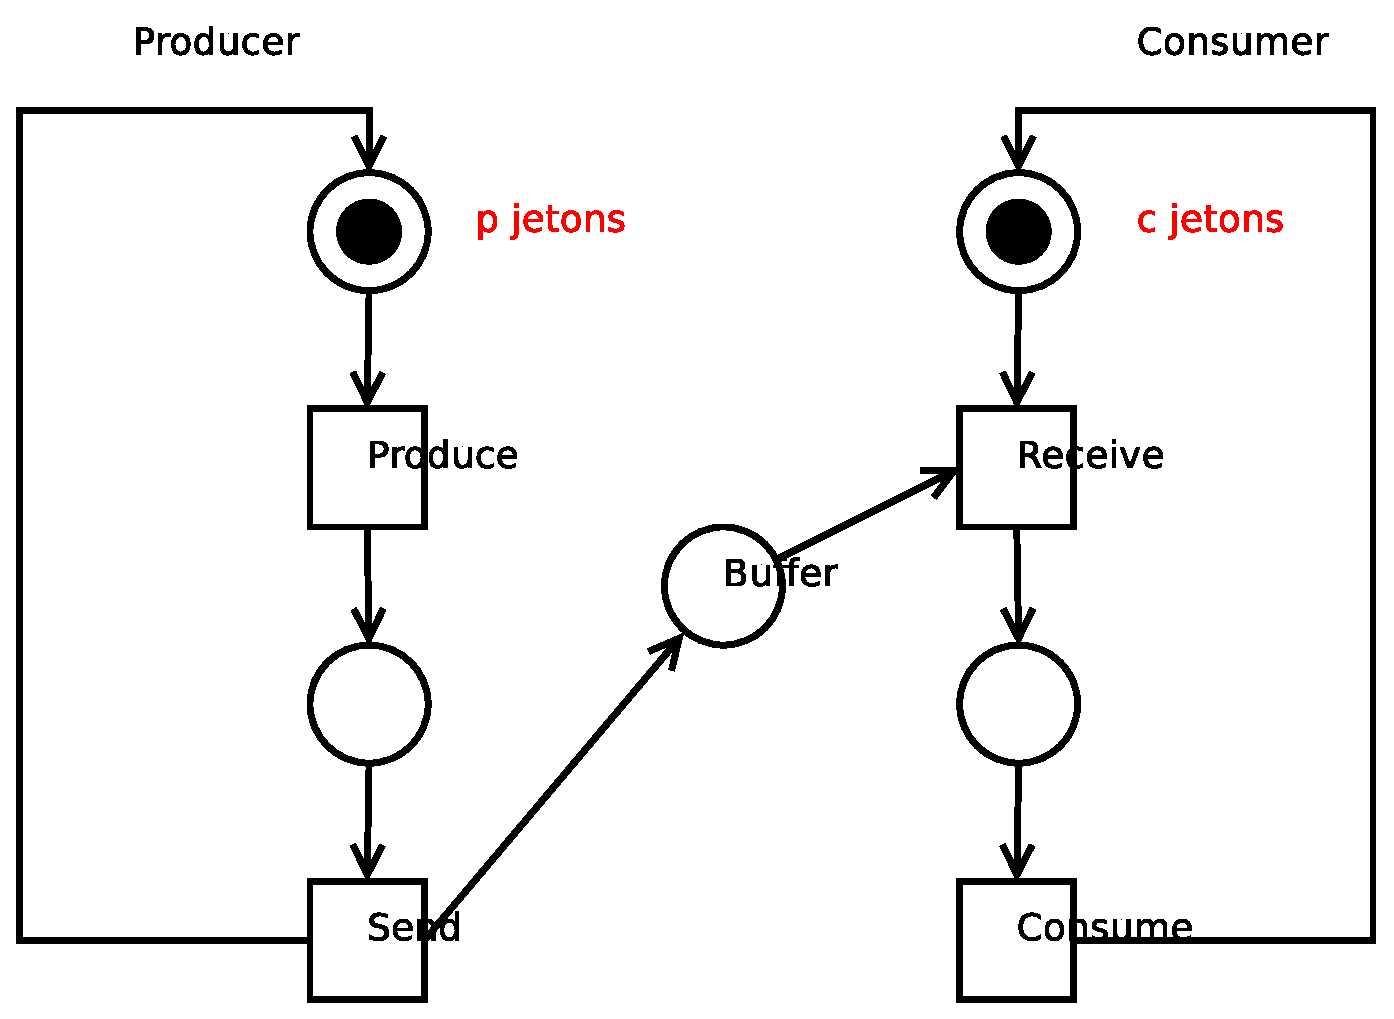
\includegraphics[height=6cm]{exo5_1.eps}
\end{center}

\subsection*{Question 2}

On rajoute un compteur de taille $b$ (et $B \leq b$) de la manière
suivante~:

\begin{center}
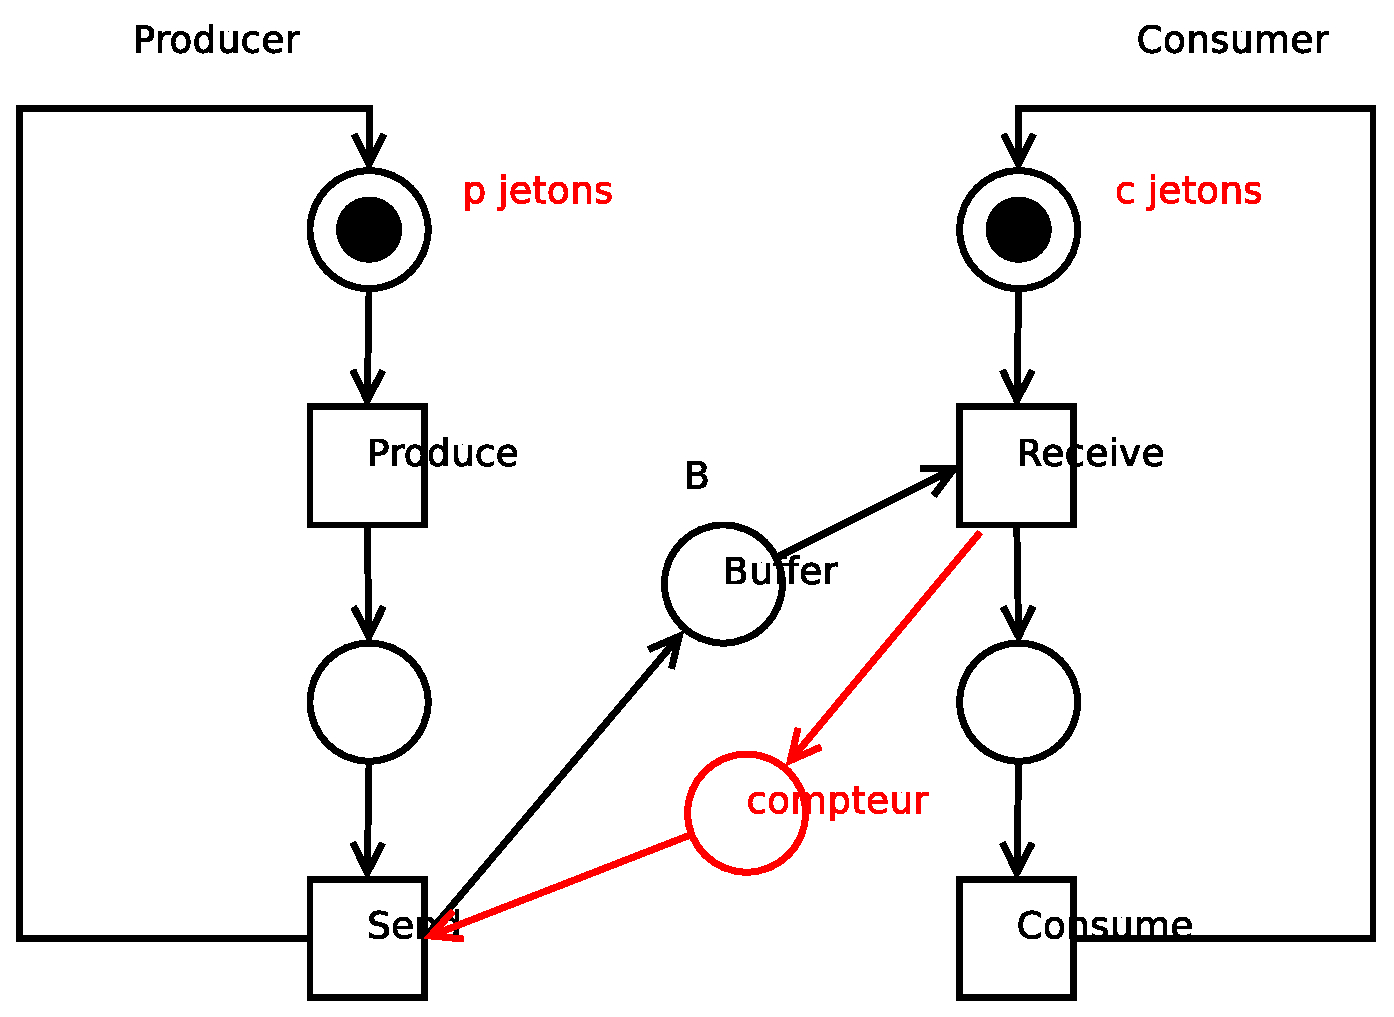
\includegraphics[height=6cm]{exo5_2.eps}
\end{center}

\subsection*{Question 3}

Pour que les messages soient reçus dans l'ordre d'envoi, il faut assigner au buffer une taille de $1$.
